\documentclass{article}
\usepackage[left=2cm, right=2cm, top=3cm, bottom=3cm]{geometry}
\usepackage[utf8]{inputenc}
\usepackage{amsmath}
\usepackage{amsthm}
\usepackage{amssymb}
\usepackage{hyperref}
\usepackage{graphicx}
\usepackage{xcolor}
\usepackage{cancel}
\usepackage{enumitem}
\usepackage{placeins}



\hypersetup{
    colorlinks,
    citecolor=black,
    filecolor=black,
    linkcolor=black,
    urlcolor=black
}

\newcommand{\R}{\mathbb{R}}
\newcommand{\N}{\mathbb{N}}
\newcommand{\Q}{\mathbb{Q}}
\newcommand{\Z}{\mathbb{Z}}
\newcommand{\Rext}{\widetilde{\mathbb{R}}}

\newcommand{\DeltaEp}{\delta_{\varepsilon}} %delta_epsilon

\newcommand{\vSpace}{\vspace{1em}}
\newcommand{\hSpace}{\hspace{1em}}

\author{A. Languasco}

\title{Teoria Analisi 1}

\begin{document}
\maketitle
\tableofcontents\newpage

\begin{flushleft}

\section{Teorema del differenziale (Lagrange - Rolle generalizzato)}
Se una funzione è derivabile in un punto, allora il suo comportamento vicino a quel punto può essere descritto da una retta tangente (approssimazione lineare). Il termine 
$o(x - x_0)$ indica che il resto dell'approssimazione tende a zero più velocemente di $x - x_0$.\\
\subsection{Enunciato}
$f: I \subset \R, I$ intervallo, $x_0 \in I$, $x_0$ interno ad $I$, $f$ derivabile in $x_0$.
\\Allora: $\exists$ w: I $\rightarrow \R$ t.c. w è continua in $x_0$, w($x_0$) = 0 e
\[
    f(x_0) + f'(x_0)(x-x_0)+w(x)(x-x_0)
\]
\\dove: $f(x_0) + f'(x_0)(x-x_0)$ è la tangente
\\\hspace{2.3em} $w(x)(x-x_0)$ è l'errore causato da alcuni fattori, \underline{lo possiamo trascurare.}

\section{! Dimostrazione}

\section{Teorema dell'unicità del limite}
\subsection{Enunciato}
$f: A \subset \R \rightarrow \R$, $x_0 \in \Rext$ punto di accumulazione per $A$
Se:
\begin{enumerate}
    \item $\lim\limits_{x \to x_0} f(x) = l_1 \in \Rext$
    \item $\lim\limits_{x \to x_0} f(x) = l_2 \in \Rext$
\end{enumerate}
Allora: $\mathbf{l_1 = l_2}$

\subsection{Dimostrazione}

\begin{enumerate}
    \item[ip1)] $\forall V l_1 $ intorno di $l_1 \exists U x_0$ intorno di $x_0$ t.c. $f(x)\in\forall l_1 $ per ogni $x\in (U x_0 \cap A) - \{0\}$
    \item[ip2)] $\forall V l_2 $ intorno di $l_2 \exists U' x_0$ intorno di $x_0$ t.c. $f(x)\in\forall l_2 $ per ogni $x\in (U' x_0 \cap A) - \{0\}$
\end{enumerate}

\begin{figure}[h]
    \centering
    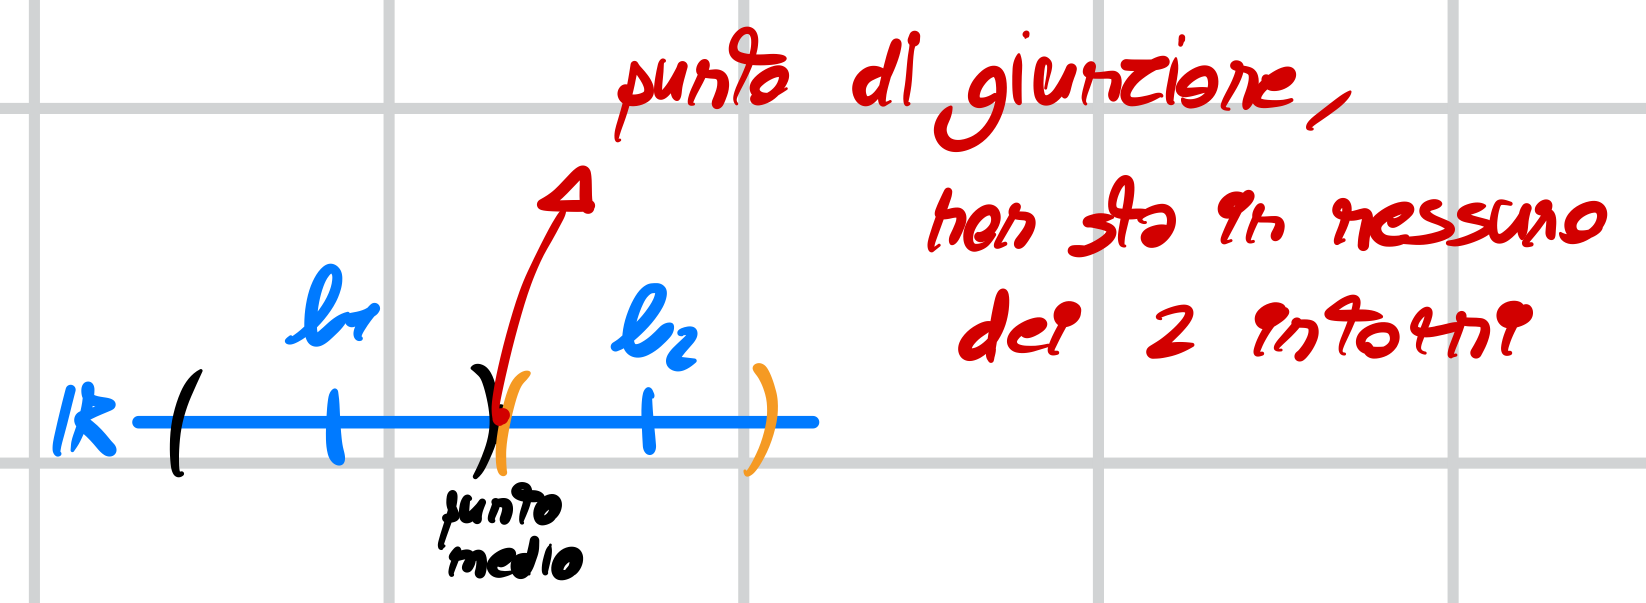
\includegraphics[width=18em]{./images/unicitaLimite.PNG}
\end{figure}

Per contraddizione: $l_1 \neq l_2$
\\Allora $\exists Vl_1, Vl_2$ intorni di $l_1$ e $l_2$ (rispettivamente) tali che: $Vl_1 \cap Vl_2 \neq \emptyset$
\\$Wx_0 = U x_0 \cap U'x_0$ è un intorno di $x_0$
\\Sia $x \in(Wx_0 \cap A) - \{x_0\} \neq \emptyset$ (perché $x_0$ è di accumulazione)
\[
    \Rightarrow
    \begin{cases}
        f(x) \in Vl_1 \text{  (Per definizione di limite 1)}\\
        f(x) \in Vl_2 \text{  (Per definizione di limite 2)}
    \end{cases}
\]
\[
    \Rightarrow f(x) \in Vl_1 \cap Vl_2 \neq \emptyset \Rightarrow \mathbf{l_1 = l_2}. \mathbf{\textbf{ \underline{Contraddizione}}}
\]
\newpage
\section{Teorema fondamentale del calcolo integrale (TFCI)} \label{TFCI}
\subsection{Enunciato}
$[a,b] \subset \R$, $a < b$. $f$ R-integrale su $[a,b]$.
\\$\exists x_1 \in [a,b]$ t.c. $f$ sia continua in $x_1$.
\\Fissato $x_0 \in $[a,b] e presa $F(x) = \int_{x_0}^{x}f(t)dt$, si ha che $F$ è derivabile in $x_1$ e $F'(x_1)=f(x_1)$
\subsection{Dimostrazione}

\begin{align*}
    0 &\leq \left| \frac{F(x) - F(x_1)}{x - x_1} - f(x_1) \right|, \quad x \neq x_1 \\
    &= \left| \frac{\int_{x_0}^{x} f(t) dt - \int_{x_0}^{x_1} f(t) dt}{x - x_1} - f(x_1) \right| \\
    &= \left| \frac{\int_{x_0}^{x} f(t) dt + \int_{x_1}^{x} f(t) dt - \int_{x_0}^{x_1} f(t) dt}{x - x_1} - f(x_1) \right| \\
    &= \left| \frac{\int_{x_1}^{x} f(t) dt - f(x_1)(x - x_1)}{x - x_1} \right| \\
    &= \left| \frac{\int_{x_1}^{x} (f(t) - f(x_1)) dt}{x - x_1} \right| \\
    &\leq \frac{1}{x - x_1} \int_{x_1}^{x} |f(t) - f(x_1)| dt
\end{align*}
\vSpace
\[ 
  \text{Ma } f \text{ è continua in }x_1 \iff \forall\epsilon>0\text{ }\exists \DeltaEp>0\text{ t.c. }\left|f(t) - f(x_1)\right|<\epsilon\text{ }\forall t / 0 < \left|t-x_1\right|<\DeltaEp\text{ }t\in[a,b]
\]

Osservo che $t\in[x_1, x]$ (oppure $t\in[x, x_1]$, dipende come abbiamo disposto $x$ e $x_1$)
\\Implica che $\left|t-x_1\right| \leq \left|x - x_1\right|$
\\Sia allora $x\in[a, b] / \left|x-x_1\right|<\DeltaEp$. \underline{Con questo forziamo le due varibli a stare vicine fra loro}
\\Quindi $\left|t-x_1\right| \leq \left|x-x_1\right|<\DeltaEp$ e $\left|f(t) - f(x_1)\right|<\epsilon$
\\Allora $0\leq\left|\frac{F(x)-F(x_1)}{x-x_1}-f(x_1)\right| < \frac{1}{\left|x-x_1\right|}\left|\int_{x_1}^{x}\epsilon dt\right| = \epsilon \frac{\left|x-x_1\right|}{\left|x-x_1\right|} = \epsilon$
\\Ossia: $\forall \epsilon > 0$ $\exists \DeltaEp > 0$ t.c. $\left|\frac{F(x)-F(x_1)}{x-x_1}-f(x_1)\right|<\epsilon$ $\forall x$ t.c. $0<\left|x-x_1\right|<\DeltaEp$, $x\in[a,b]$
\\Cioè:$\lim_{x_1}\frac{F(x)-F(x_1)}{x-x_1}$ esiste e vale $f(x_1)$.
\\\begin{center} \textbf{Quindi: $\mathbf{F'(x_1) = f(x_1)}$}\end{center}

\newpage
\section{Formula fondamentale del calcolo integrale}
\subsection{Enunciato}
$f \in C^0[a,b]$ e sia $G : [a,b] \rightarrow {\R}$ una primitiva di $f$ in $[a,b]$
\\\begin{center}$\Rightarrow \int_{a}^{b}f(t)dt = G(b) - G(a)$\end{center}

\subsection{Dimostrazione}
Sia $x \in [a,b]$ e $F(x)= \int_{x_0}^{x}f(t)dt$. Per il TFCI* è derivabile in $[a,b]$ e $F'(x)=f(x) \forall x \in [a,b]$.
\\$F$, $G$ sono primitive di $f$ in un intervallo $[a,b] \Rightarrow$ $\exists c \in {\R} /G(x)=F(x)+c$ $\forall x \in [a,b]$
\begin{center}
    Osservo adesso che: $G(b) - G(a) = F(b)+c-F(a)-c=F(b)-F(a)$
    \\$= \int_{x_0}^{b}f(t)dt - \int_{x_0}^{a}f(t)dt$
    \\$= \cancel{\int_{x_0}^{a}f(t)dt} + \int_{x_0}^{b}f(t)dt - \cancel{\int_{x_0}^{a}f(t)dt} = \int_{x_0}^{b}f(t)dt$.
\end{center}
*TFCI: \hyperref[TFCI]{Teorema Fondamentale Calcolo Integrale}
\vSpace
\\\underline{\textbf{Osservazione:}} $f \in C^0 ([a,b])$ e sia
\\$H(x) = \int_{\alpha(x)}^{\beta(x)}f(t)dt$ dove $\alpha,\beta:[a,b]\rightarrow \R$ derivabili in $[a,b]$.
\\Si ha che $H(x)$ è derivabile perché $H(x)=F(\beta(x))-F(\alpha(x))$ dove $F(u)=\int_{x_0}^{u}f(t)dt$ \textit{(Composizione di $f$ derivabili)}
\\Inoltre $H'(x)=F'(\beta(x))\beta'(x) - F'(\alpha(x))\alpha'(x) = $ \underline{$f(\beta (x))\beta'(x)-f(\alpha(x))\alpha'(x)$ $\forall x \in [a,b]$}


\section{Teorema del confronto I}
\subsection{Enunciato}
$f, g: A \subset \R \rightarrow \R, x_0 \in \Rext$ punto di accumulazione per $A$
\\Allora: 

\begin{enumerate}
    \item[a)] Se \( \lim\limits_{x \to x_0} f(x) = \ell_1 \in \mathbb{R} \) \\
          Se \( \lim\limits_{x \to x_0} g(x) = \ell_2 \in \mathbb{R} \) \\
          con \( \ell_1 < \ell_2 \), allora:
          \[
          \exists U_{x_0}, \text{ intervallo di } x_0, \text{ tale che } f(x) < g(x) \quad \forall x \in (U_{x_0} \cap A) \setminus \{x_0\}
          \]
    
    \item[b)] Se \( \lim\limits_{x \to x_0} f(x) = -\infty \) \\
          Se \( \lim\limits_{x \to x_0} g(x) = \ell \in \mathbb{R} \cup \{+\infty\} \), allora:
          \[
          \exists U_{x_0}, \text{ intervallo di } x_0, \text{ tale che } f(x) < g(x) \quad \forall x \in (U_{x_0} \cap A) \setminus \{x_0\}
          \]

    \item[c)] Se \( \lim\limits_{x \to x_0} f(x) = \ell \in \mathbb{R} \) \\
          Se \( \lim\limits_{x \to x_0} g(x) = +\infty \), allora:
          \[
          \exists U_{x_0}, \text{ intervallo di } x_0, \text{ tale che } f(x) < g(x) \quad \forall x \in (U_{x_0} \cap A) \setminus \{x_0\}
          \]
\end{enumerate}

\subsection{Dimostrazione}
\begin{enumerate}
    \item[a)]
    $l_1 < l_2 (l_1,l_2 \in \R)$. Fisso $\epsilon>0$\\
    $\lim\limits_{x \to x_0} f(x)=l_1 \Rightarrow \exists U' x_0$ intervallo di $x_0$ tale che $\forall x \in (U' x_0 \cap A)\setminus \{x_0\}$
    \\$\lim\limits_{x \to x_0} g(x) = l_2 \Rightarrow \exists U'' x_0$ intorno di $x_0 / l_2 - \epsilon < g(x) < l_2 + \epsilon$ $\forall x \in (U'' x_0 \cap A) \setminus \{x_0\}$
    \vSpace
    \\Se $x \in (U' x_0 \cap U'' x_0 \cap A) \setminus \{x_0\}$ \textit{idea: scelgo $\epsilon>0 / l_1 + \epsilon \leq l_2 - \epsilon$}
    \\Scelgo in quanto sopra $\epsilon = \frac{l_2 - l_1}{2}$
    \\Per $x \in (U' x_0 \cap U'' x_0 \ cap A) \setminus \{x_0\}$ si ha allora 
    \[f(x) < l_1 + \epsilon = l_1 + \frac{l_2 - l_1}{2} = \frac{l_1 + l_2}{2}\]
\end{enumerate}


\section{Teorema del confronto II}
\subsection{Enunciato}
$f, g: A \subset \R \rightarrow \R$ $A \neq \emptyset$ $x \in \Rext$ punto di accumulazione per $A$ Allora:
\begin{enumerate}
        \item[a)]
        Se $\lim\limits_{x \to x_0} f(x) = l_1 \in \R$
        \\Se $\lim\limits_{x \to x_0} g(x) = l_2 \in \R$
        \\Se $\exists U x_0$ intorno di $x_0 / f(x) \leq g(x)$ $\forall x \in (U x_0 \cap A)\setminus \{x_0\}$
        \[\Rightarrow l_1 \leq l_2\]

        \item[b)]
        Se $\lim\limits_{x \to x_0} g(x) = - \infty$ e $\exists U x_0$ intorno di $x_0 / f(x) \leq g(x)$ $\forall x \in (U x_0 \cap A) \setminus \{x_0\}$
        \[ \Rightarrow \exists \lim\limits_{x \to x_0} g(x) = + \infty \]

        \item[c)]
        Se $\lim\limits_{x \to x_0} f(x) = + \infty$ e $\exists U x_0$ intorno di $x_0 / f(x) \leq g(x)$ $\forall x \in (U x_0 \cap A) \setminus \{x_0\}$
        \[ \Rightarrow \exists \lim\limits_{x \to x_0} g(x) = + \infty \]
\end{enumerate}
\subsection{Osservazione}
Cosa accade se si suppone $f(x) < g(x) \overset{?}{\Rightarrow} l_1 < l_2$
\[ 
    \textbf{NO: } f(x)=0 \text{ } \forall x \R \text{ } g(x) = 
    \begin{cases}
        \frac{1}{x} \text{ } x > 0\\
        0 \text{ } x = 0\\
        - \frac{1}{x} \text{ } x < 0
    \end{cases}
\]

\begin{figure}[h]
    \centering
    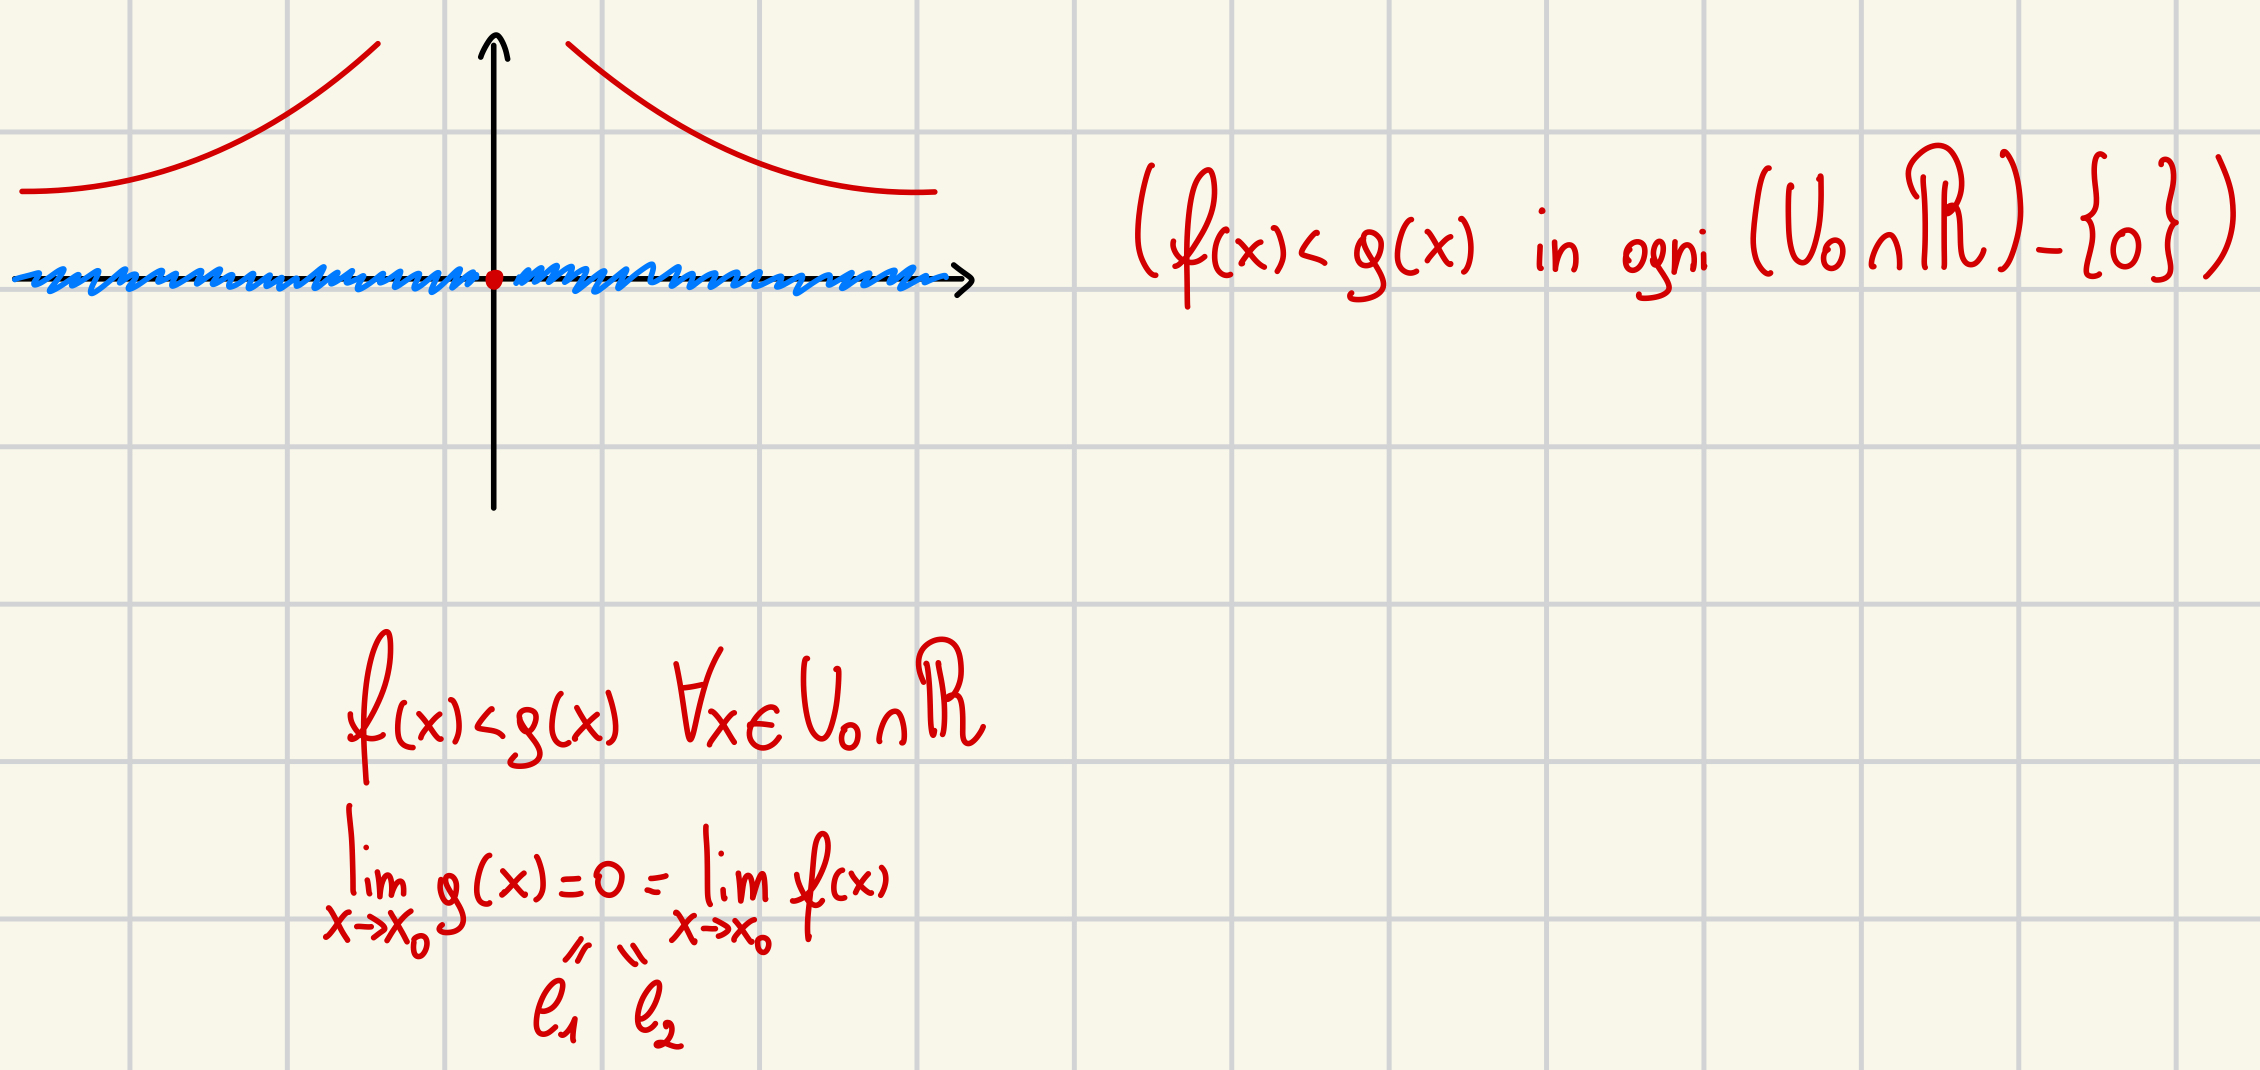
\includegraphics[width=22em]{./images/Teoriaconfronto2.jpeg}
\end{figure}

\newpage
\section{Teorema del confronto III - delle 3 funzioni - Carabinieri}

\includegraphics[width = 5em]{./images/carabinieri.png}
\subsection{Enunciato}
$f, g, h:$ $A \subset \R \rightarrow \R,$ $A \neq \emptyset,$ $x_0 \in \Rext$ punto di accumulazione per $A$.
\\Inoltre
\begin{enumerate}
    \item[] $\exists \lim\limits_{x \to x_0} f(x) = l \in \R$ 
    \item[] $\exists \lim\limits_{x \to x_0} g(x) = l \in \R$
    \item[] $\exists U x_0$ intorno di $x_0 / f(x) \leq h(x) \leq g(x)$ $\forall x \in (U x_0 \cap A) \setminus \{x_0\}$
\end{enumerate}
\[ \Rightarrow \exists \lim\limits_{x \to x_0} h(x) = l \]


\subsection{Dimostrazione}
Sia $\epsilon > 0$: $\exists U' x_0$, $U'' x_0$ intorni di $x_0 / \left|f(x) - l\right| < \epsilon$  $\forall x \in (U' x_0 \cap A) \setminus \{x_0\}$
\\\hspace*{16.32em} $\left|g(x) - l\right| < \epsilon$  $\forall x \in (U'' x_0 \cap A) \setminus \{x_0\}$
\\\vSpace Sia $W x_0 = U' x_0 \cap U'' x_0$ è un intorno di $x_0$.
\\Se $x \in W x_0 \cap A \setminus \{x_0\}$
\vSpace
\\\hspace*{18em}$l - \epsilon < f(x)$ \underline{definizione $\lim f$ (per ipotesi)}
\\\hspace*{18em}\hspace*{3.3em}$f(x) \leq h(x) \leq g(x)$
\\\hspace*{18em}\hspace*{9.8em}$g(x) < l + \epsilon$
\vSpace
\\Quindi $l - \epsilon < h(x) < l + \epsilon$ cioè $\left|h(x) - l\right| < \epsilon$
\\Ho fatto vedere che:
\[
    \forall \epsilon > 0 \text{ } \exists W x_0 \text{ intorno di } x_0 / \left|h(x) - l\right| < \epsilon \text{ per } x \in W x_0 \cap A \setminus \{x_0\}
\]
\\Che è esattamente la definizione di: $\lim\limits_{x \to x_0} h(x) = l$

\newpage
\section{Teorema del valore medio integrale}
\subsection{Enunciato}
$f: [a,b] \rightarrow \R$, $f, g R-integrale in [a,b]$.\\
Sia $m = $inf${f(x) / x \in [a,b]}$, $(\in \R)$\\
\hspace*{1.15em} $M = $sup${f(x) / x \in [a,b]}$, $(\in \R)$\\
\vSpace
\[
    \Rightarrow
    \begin{cases}
        $1) $m(b-a) \leq \int_{a}^{b} f(x) dx \leq M(b-a)\\
        $2) $\exists \mu \in [m,M] / \int_{a}^{b}f(x)dx = \mu (b-a)\\
        $3) Se $f$ continua in $[a,b]$, allora $\exists x_0 \in [a,b] / \int_{a}^{b}f(x)dx = f(x_0)(b-a).
    \end{cases}
\]
\subsection{Dimostrazione}
1) $m \leq f(x) \leq M$ $x \in [a,b]$\\
\hspace*{1.2em}$P = {a,b} \Rightarrow D(P, f) = m (b-a) \in G$\\
\hspace*{1.2em}\hspace*{5em}$S'(P, f) = M(b-a) \in H$.\\
\hspace*{1.2em}Allora: $m(b-a) \leq sup(G) = \int_{a}^{b}f(x)dx = inf(H) \leq M(b-a)$\\
\vSpace
2) Dal punto 1): $m \leq \frac{\int_{a}^{b}f(x)dx}{b-a} \leq M.$ Sia $\mu = \frac{\int_{a}^{b}f(x)dx}{b-a}$,\\
\hspace*{1.2em}allora $\mu \in [m,M]$ e ovviamenete, $\int_{a}^{b}f(x)dx = \mu (b-a)$
\\\vSpace
3) $f \in C^0[a,b]: $ per il teorema dei valori intermedi $f([a,b])$ è intervallo; per il teorema di Weistrass $f$ ha max e min \textbf{GLOBALE}\\
\hspace*{1.2em}Quindi $f([a,b]) = [m, M]$\\
\hspace*{1.2em}Per il punto 2), $\exists \mu \in [m,M] / \mu (b-a) = \int_{a}^{b}f(x)dx$;\\
\hspace*{1.2em}ma $[m,M] = Im(f) \Rightarrow \exists x_0 \in [a,b] / f(x_0) = \mu$ 

\section{Criterio integrale convergenza delle serie numeriche}
\subsection{Enunciato}
$f: [1, + \infty ) \rightarrow \R,$ $f(x) \geq 0$ $\forall x \in [1, + \infty)$.
\\Sia $f$. debolmente crescente in $[\, + \infty )$.
\\Allora ($\sum\limits_{k=1}^{\infty} f(k)$ converge $\iff$ $\int_{1}^{+ \infty} f(x) dx$ converge.)

\section{Teorema delle derivate successive}
\subsection{Enunciato}
Sia $n \in \N$, $n \geq 1$, $f \in C^{n-1}(I)$, $I$ intervallo, $x_0 \in I$, $x_0$ interno ad $I$.\\
Suppongo che $\exists f^n(x_0)$ e che $f^{(k)}(x_0)=0$ per $k = 1, 2, 3, ..., n-1$.\\
\hspace*{12.7em}$f^{(n)} > 0$ $(<0)$.\\
\[
    \Rightarrow
    \begin{cases}
        $se $n$ è \textbf{PARI}, si ha che $x_0$ è punto di minimo (massmimo) locale forte.$\\
        $se $n$ è \textbf{DISPARI}, allora $x_0$nè pto di massimo nè pto di minimo locale.$
    \end{cases}
\]


\section{Teorema di Rolle} \label{Rolle}
\subsection{Enunciato}
$f:[a,b] \rightarrow \R$, $f$ continua in $[a,b]$
\\$f$ derivabile in $(a,b)$ e $f(a) = f(b)$
\\Allora $\exists \overline{x} \in [a,b]$
\\\underline{$x_1 = a$ e $x_2 = b$ (o viceversa)}: allora, dato che
\[
    \begin{array}{c}
        f(a) = f(b) \Rightarrow f(x) = f(a) \text{ } \forall x \in [a,b] \\
        \Rightarrow f'(x) = 0 \text{ } \forall x \in (a,b)
    \end{array}
\]
Se almeno uno tra $x_1$ e $x_2$ non è in un estremo di $[a,b]$
\\esempio sia $x_1 \in (a,b)$. Allora $x_1$ è interno ad $[a,b]$. Per le condizioni necessarie di estremalità si ha $f'(x_1) = 0$
\\Nel caso di $x_2 \in (a,b)$: si replichi lo stesso ragionamento.

\section{Teorema di Lagrange}
\subsection{Enunciato}
$f:[a,b] \rightarrow \R$, $f$ continua in $[a,b]$, $f$ derivabile in $(a,b)$.
\[ \Rightarrow \exists \overline{x} \in (a,b) / f(b) - f(a) = f'(\overline{x}) (b-a)\]

\subsection{Dimostrazione}
Sia $\varphi (x) = (f(x)- f(a))(b - a) - (f(b) - f(a))(x-a)$, $f$ è continua in $[a,b]$;
\\$\varphi$ è derivabile in $(a,b)$, $\varphi (a) = 0 - 0 = 0$; $\varphi (b) = 0 - 0 = 0$.
\\Per il teorema di \hyperref[Rolle]{Rolle}: $\exists \overline{x} \in (a,b)$ \hspace*{2em} $\varphi (\overline{x}) \rightarrow$ punto che azzera la derivata prima.
\\Ma $\varphi ' (x) = (f'(x)(b-a)) - (f(b)-f(a))$ $\forall x \in (a,b)$
\[
    \begin{array}{c}
        \Rightarrow 0 = \varphi ' (\overline{x}) = f'(\overline{x})(b-a) - f(b)-f(a) \\
        \text{e quindi } 0 = \varphi ' (\overline{x}) \text{ dato che il resto è nullo}\\
        \text{da cui segue la tesi.}
    \end{array}
\]

\begin{figure}[h]
    \centering
    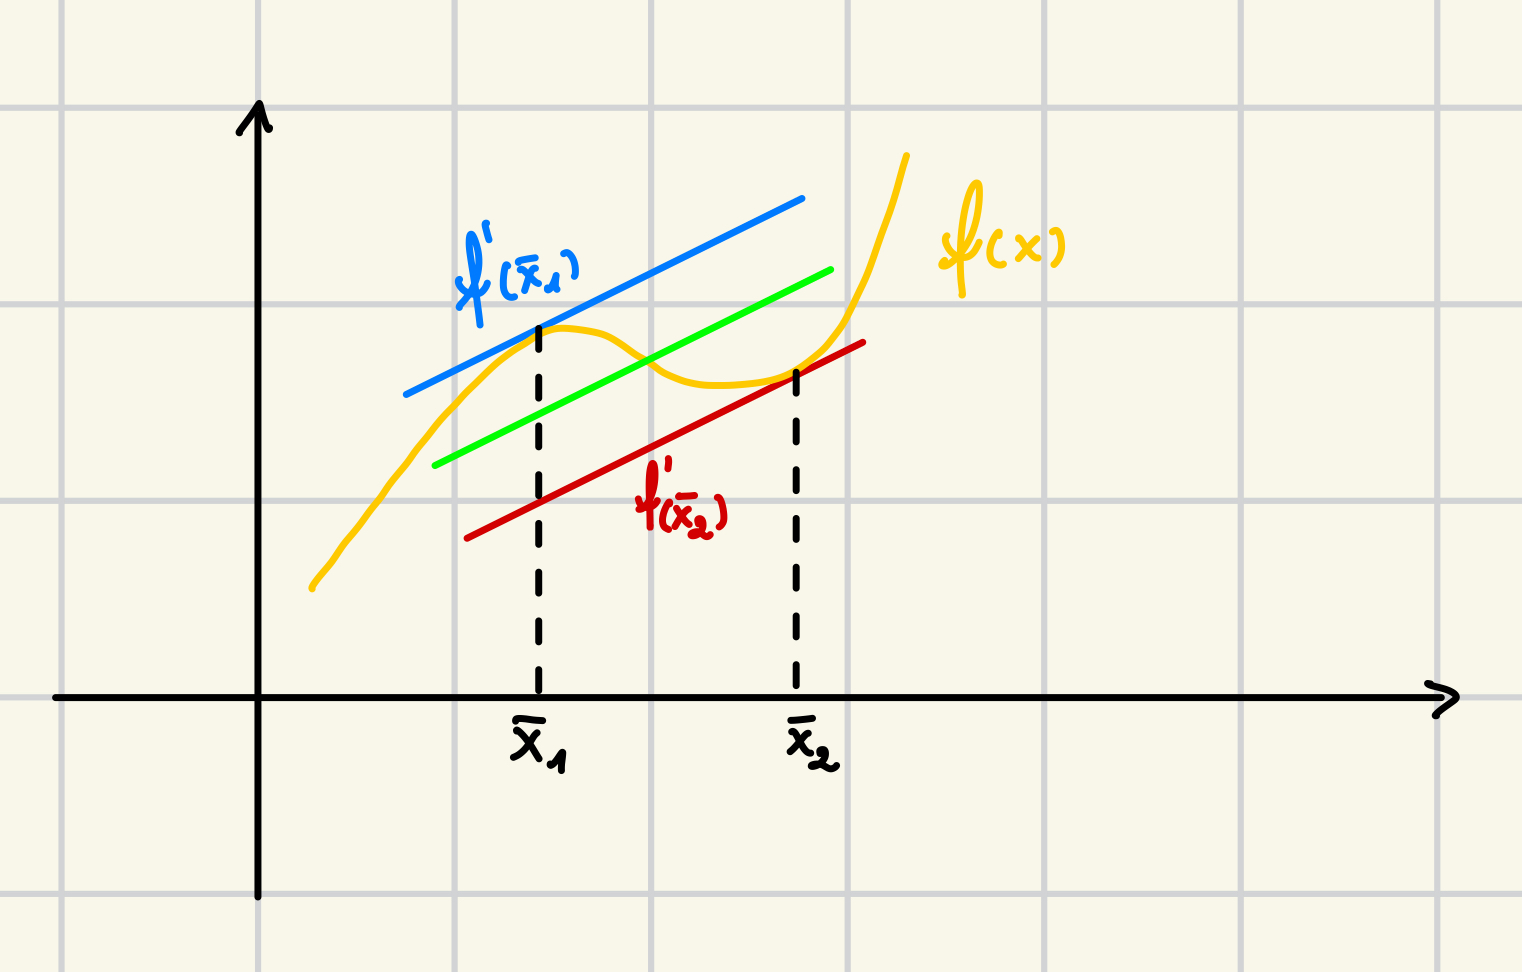
\includegraphics[width=25em]{./images/lagrange.jpeg}
\end{figure}
\FloatBarrier


\section{Teorema condizione necessaria di convergenza delle serie}
\subsection{Enunciato}
\[
\text{Se } \sum a_k \text{ converge, allora } \lim\limits_{x \to + \infty}a_k = 0
\]

\subsection{Dimostrazione}
Sia $A_n = \sum\limits_{k = 0}^{n}a_n$, $n \in \N$.\\
Per ipotesi $\exists A \in \R \lim\limits_{n \to + \infty} An = A$. \\
Inoltre si ha che $A_n - A_{n-1} = \sum\limits_{k = 0}^{n}a_n - \sum\limits_{h = 0}^{n-1}a_n = a_n$
\\Ma $\lim\limits_{n \to + \infty}(A_n - A_{n-1}) = (\lim\limits_{n \to + \infty}A_n) - (\lim\limits_{n \to + \infty}A_{n-1}) = A - A = 0$
\[
\Rightarrow \lim\limits_{n \to + \infty}a_n = 0\text{.}
\]

\section{Teorema Disuguaglianza di Bernoulli}
\subsection{Enunciato}
$x \in \R$, $x > - 1$. Allora $(1+x)^m \geq 1 + nx$ $\forall n \in \N$

\subsection{Dimostrazione}
\textbf{Passo base:}\\
È vero che: $(1+x)^0 \leq 1 + 0 * x?$, si $\Rightarrow$ passo base \underline{verificato!}
\\\vSpace
\textbf{Passo induttivo:}\\
Ipotesi induttiva: $(1+x)^m \geq 1 + mx$ \hspace*{1em} con $m \in \N$\\
Tesi induttiva: $(1+x)^{m+1} \geq \textcolor{red}{1 + (m+1)x}$
\\\vSpace
$(1+x)^{m + 1} = (1+x)(1+x)^m \geq (1 + mx)(1+x)$\\
$1 + x + mx + mx^2 = x(1+m)+ 1 + mx^2 = (m+1)x + 1 + mx^2 \geq \textcolor{red}{(m+1)x + 1}$ \hspace*{1em}Posso anche ingnorare $mx^2$ perche è sempre positivo
\\\vSpace
\textbf{Quindi il passo induttivo è verificato per il principio di induzione $\forall x > -1$}

\newpage
\section{Integrale di Riemann}
\subsection{Integrali Definiti}
Vogliamo dare un significato al concetto (per $f(x) \geq$ 0) di "area sottesa al grafico di $f$".

\begin{figure}[h]
    \centering
    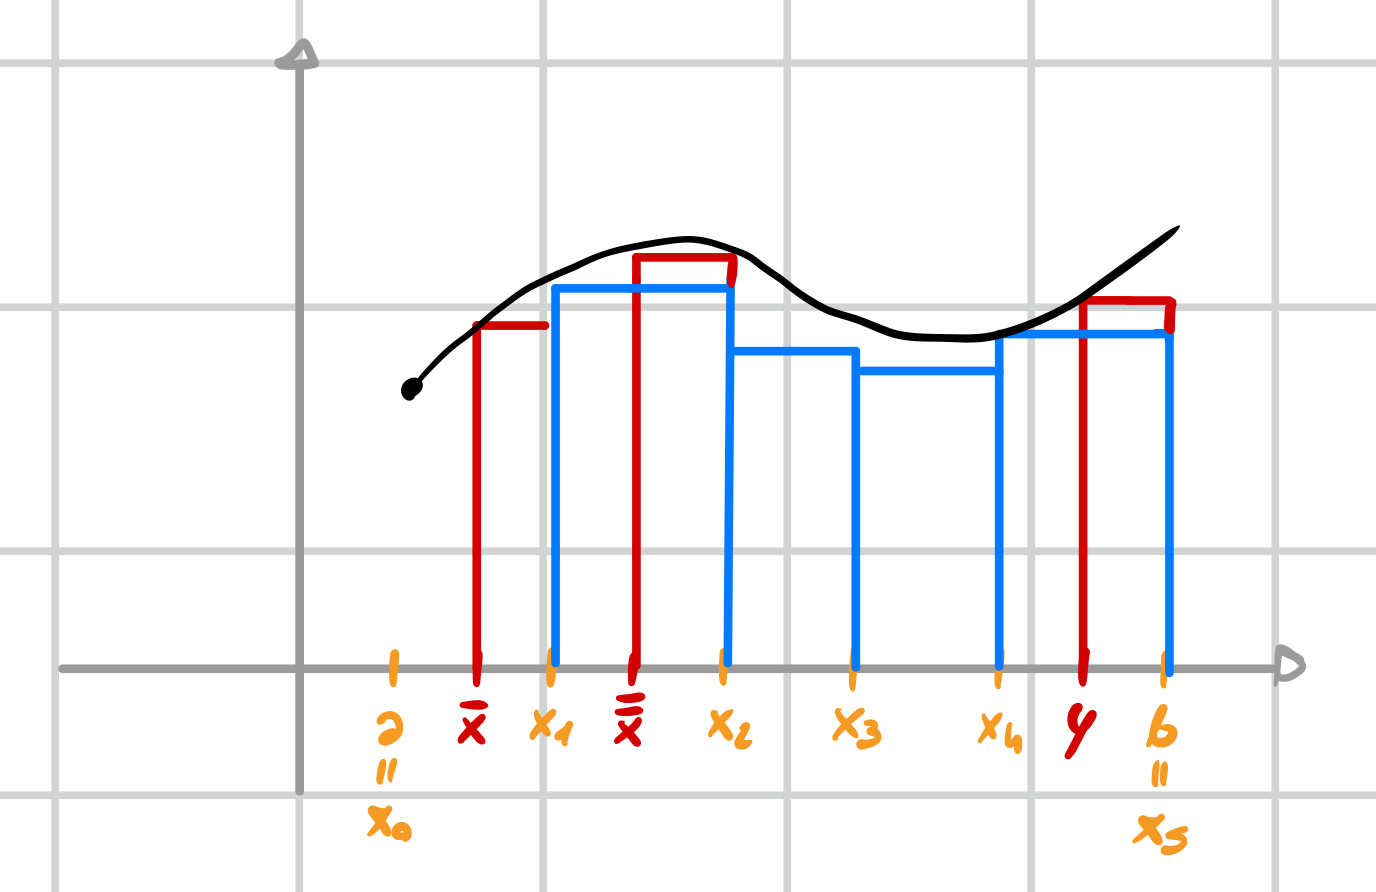
\includegraphics[width=20em]{./images/riemann.png}
\end{figure}
\FloatBarrier

\subsection{Estensione dell'integrale di Riemann}
A casi cui $a \geq b$.

\begin{figure}[h]
    \centering
    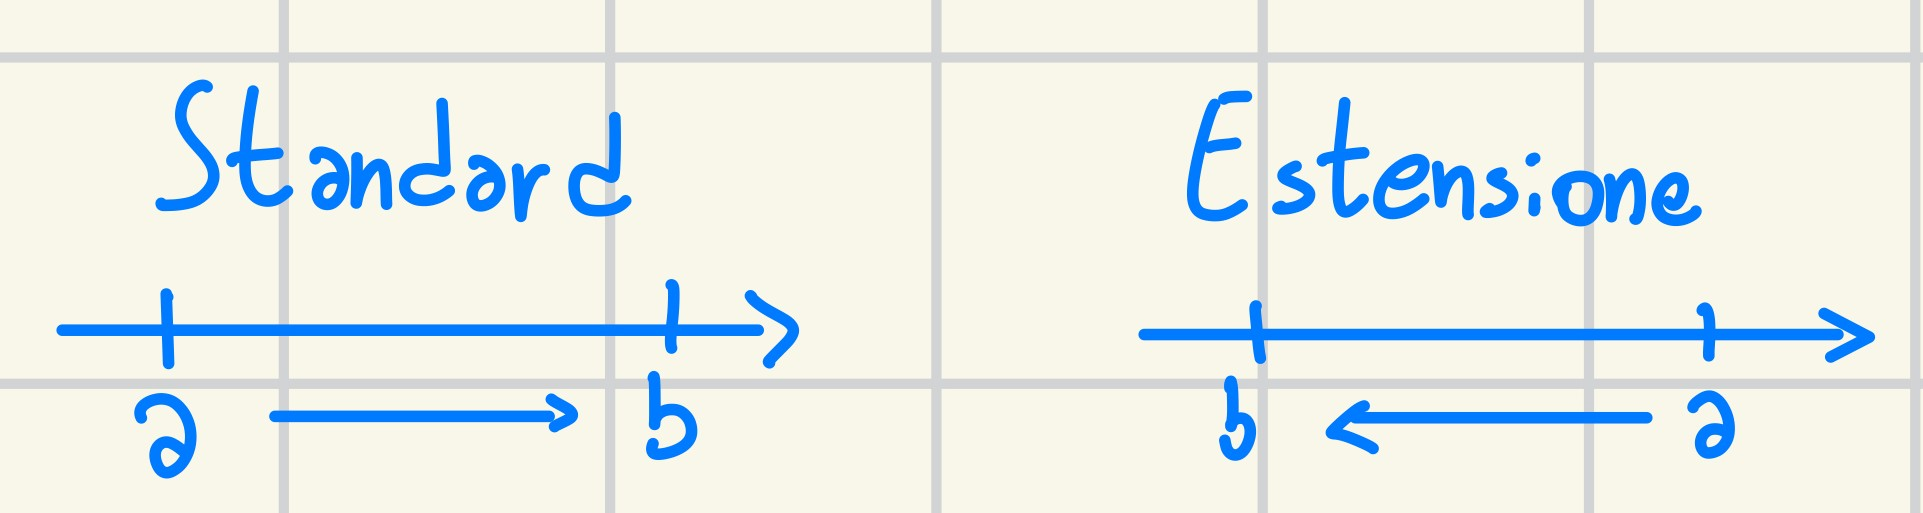
\includegraphics[width=20em]{./images/riemann_extension.jpeg}
\end{figure}
\FloatBarrier

\subsubsection{Definizione}
$f$ Riemann-integrale in $[a,b]$, $a < b$, $a, b \in \R$.\\
\[
    \text{Definiamo }\int_{a}^{b}f(x)dx = 0\text{ e }\int_{b}^{a}f(x)dx = \mathbf{ - \int_{a}^{b}f(x)dx}
\]

\subsection{Teorema Integrazione di Riemann per parti}
$f, g: [a,b] \rightarrow \R $, $f, g \in C^1([a,b])$\\
\[
    \text{Allora: } \int_{a}^{b}f(x)g'(x)dx =\textcolor{orange}{ f(b)g(b) - f(a)g(a)} - \int_{a}^{b}f'(x)g(x)dx
\]

$\textcolor{orange}{ f(b)g(b) - f(a)g(a)} = f(x)g(x)|_{a}^{b}$

\subsubsection{Dimostrazione}
$f'g$ e $fg'$ sono continue in $[a,b]$ e quindi sono R-int$^\text{le}$ in $[a,b]$.\\
Inoltre $\int_{a}^{b}(fg)'(x)dx = \int_{a}^{b}f'(x)g(x)dx + \int_{a}^{b}f(x)g'(x)dx$\\
Ma  f*g è primitiva di  $(fg)'$ e quindi
\[
    \int_{a}^{b}(fg)'(x)dx = f(b)g(b) - f(a)g(a) \text{ la tesi segue}
\]


\section{Teorema di Bolzano - Weierstr\ss}
\subsection{Enunciato}
Sia ${a_n}$ una successione LIMITATA (Quindi superiormente e inferiormente limitata).\\
Allora $\exists \{ a_{n_k} \}$ successione di $a_n$ t.c. 
\[\lim\limits_{k \to + \infty } a_{n_k} = l \in \R\]

\subsection{Esempio 1}
\[
    a_n  =
    \begin{cases}
        0 $ se $ n $ pari$\\
        n $ se $ n $ dispari$
    \end{cases}
\]
Sup\{$a_n$\} = $+ \infty \Rightarrow$ non posso applicare il teorema di Bolzano-Weistra\ss.

\subsection{Esempio 2}
\[
    a_n = (-1)^n \Rightarrow \left|a_n\right| \leq \text{ } \forall n \in \N
\]
Per il teorema di Bolzano-Weistra\ss $ \text{ } \exists a_{n_k}$ sottosuccessione di $a_n$ t.c. $\exists \lim\limits_{k \to + \infty} a_{n_k} \in \R$

\section{Proprietà di Archimede} \label{Archimede}
\subsection{Enunciato}
\[ \forall x \in \R \text{ } \exists n \in \N / n < x \]
"Esiste sempre un numero intero più grande di qualsiasi numero reale".
\subsection{Dimostrazione}
Sia $x>0 \rightarrow A:=\{n \in \N / n \leq x\}\subseteq \N$\\
Tesi: $\iff A \neq \N$\\

\vSpace
Suppongo che $A = \N \neq \emptyset$\\
Sia $B := \{y \in \R / y \geq n$ $ \forall n \in \N\}$\\
dal fatto che $A = \N$ segue che $x \in B \Rightarrow B \neq \emptyset$\\
Notiamo che $\forall y \in B$ si ha che $y \geq n$ $\forall n \in A (= \N)$. Quindi $A$ e $B$ sono separati per l'assioma di separazione\\
$\exists \alpha \in \R / n \leq \alpha \leq y$ $\forall n \in A$ $\forall y \in B$ \vspace*{1em} $(A = \N)$\\
Quindi è anche vero che $\N \ni n+1 \leq \alpha \leq y \Rightarrow n \leq \alpha - 1$ $\forall n \in A \Rightarrow \alpha - 1 \in B$\\
Ma $\alpha$ è elemento separatore  di $A$ e $B$: $(n \leq ) \alpha \leq y $ $\forall y \in B$ $\forall n \in A$\\
\[\text{Quindi }\alpha \leq \alpha - 1 \Rightarrow 1 \leq 0 \rightarrow \text{\textbf{Contraddizione}}\]
Abbiamo provato l'applicazione contronominale; quindi il teorema è dimostrato.\\
$A = \N$ FALSO $\Rightarrow a \subsetneq \N$

\section{Teorema Bernoulli - de l'Hopital}
\subsection{$\frac{0}{0}$; limiti al finito}
$a, b \in \R$, $f, g:(a,b) \rightarrow \R$, $f,g $ derivabili in $(a,b)$\\
\underline{$g'(x) \neq 0$} $\forall x \in (a,b)$. Siano $\lim\limits_{x \to a^+}g(x)$ e sia $\lim\limits_{x \to a^+}\frac{f'(x)}{g'(x)} = l \in \Rext$.\\
\[ \Rightarrow \lim\limits_{x \to a^+}\frac{f(x)}{g(x)} = l\]
\underline{Nota} vale anche per: $x \rightarrow b^-$, $Df = Dg = (a,b) \setminus \{x_0\}$

\subsubsection{Errori comuni}
1) \underline{\textbf{Errore:}} uguagliare $\frac{f(x)}{g(x)}$ con $\frac{f'(x)}{g'(x)}$ \underline{senza aver verificato che l'ultimo limte esiste.}\\
2) Non si può usare il teorema di Bernoulli - de l'Hopital per studiare $\lim\limits_{x \to 0}\frac{\text{sin}x}{x}$

\subsection{$\frac{0}{0}$; limiti all'infinito}
Sia $a \in \R$, $f,g: (a, + \infty)$*$ \rightarrow \R$, $f, g$ derivabili in $(a, + \infty)$* e $g'(x) \neq 0$ $\forall x \in (a, + \infty)$*\\
\textit{*$(a, +\infty)$ al contrario vale anche: $(- \infty, a)$.}\\
Inoltre $\lim\limits_{x \to + \infty}f(x) = 0 = \lim\limits_{x \to + \infty}g(x)$ e $\lim\limits_{x \to +\infty}\frac{f'(x)}{g'(x)} =l \in \Rext$.\\
\[ \Rightarrow \lim\limits_{x \to +\infty}\frac{f(x)}{g(x)} = l\]

\subsection{$\frac{\infty}{\infty}$; limiti al finito}
$a, b \in \R$, $f, g:(a,b) \rightarrow \R$, $f,g $ derivabili in $(a,b)$\\
$g'(x) \neq 0$ $\forall x \in (a,b)$. Inoltre\\
$\lim\limits_{x \to a^+}g(x) = +\infty$*; $\lim\limits_{x \to a^+}\frac{f'(x)}{g'(x)} = l \in \Rext$.\\
\textit{*$+\infty$ al contrario vale anche: $-\infty$}\\
\[ \Rightarrow \lim\limits_{x \to a^+}\frac{f(x)}{g(x)} = l\]

\subsection{$\frac{\infty}{\infty}$; limiti al'infinito}
Sia $a \in \R$, $f,g: (a, + \infty) \rightarrow \R$, $f, g$ derivabili in $(a, + \infty)$ e $g'(x) \neq 0$ $\forall x \in (a, + \infty)$.\\
Inoltre $\lim\limits_{x \to + \infty}g(x) = +\infty$*; $\lim\limits_{x \to +\infty}\frac{f'(x)}{g'(x)} = l \in \Rext$.\\
\textit{*$+\infty$ al contrario vale anche: $-\infty$}\\
\[ \Rightarrow \lim\limits_{x \to +\infty}\frac{f(x)}{g(x)} = l\]

\newpage
\section{Teorema Densità di $\Q$ in $\R$}
\subsection{Enunciato}
Per ogni $x \in \R$ e $\forall \epsilon > 0 $, $\exists z \in \Q / z \leq x < z + \epsilon$ 
\begin{figure}[h]
    \centering
    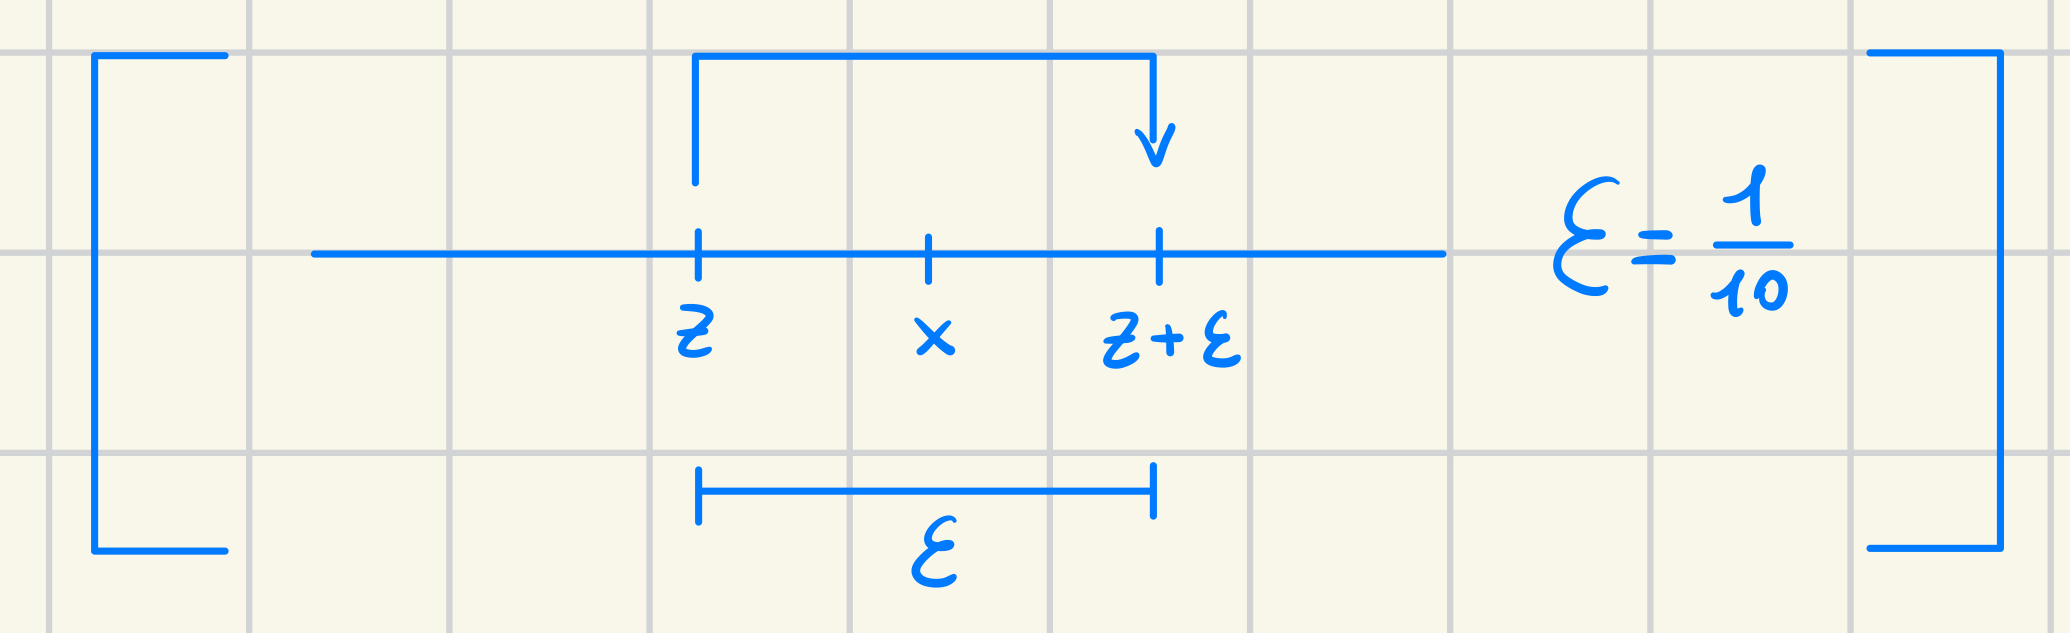
\includegraphics[width=25em]{./images/densityQinR.jpeg}
\end{figure}
\FloatBarrier

\subsection{Dimostrazione}
$x \in \R$, $\epsilon > 0 \Rightarrow \frac{1}{\epsilon}> 0$\\
Uso la \hyperref[Archimede]{Proprietà di Archimede}: $\exists q \in \N / q > \frac{1}{\epsilon} > 0$\\
Considero $qx \in \R$\\
Per le prorietà delle parti intrere $\exists p \in \Z / p \leq qz < p + 1$\\
Divido per $q > 0 \Rightarrow \frac{p}{q} \leq x < \textcolor{orange}{\frac{p + 1}{q}}$ \hspace*{1em} con
$\textcolor{orange}{\frac{p + 1}{q}} = \frac{p}{q} + \frac{1}{p}$\\
Ma $q > \frac{1}{\epsilon} = \epsilon q > 1 \Rightarrow \epsilon < \frac{1}{q}$\\
\[ \text{Segue che }\frac{p}{q}\leq x < \frac{p}{q} + \epsilon\]

\section{Definizione di Limite}
$f:A \subset \R \rightarrow \R$, $A \neq \emptyset$. Sia $x_0 \in \Rext$ un punto di accumulazione per $A$.\\
Diremo che $f$ ammette limite $l \in \Rext$ per $x$ che tende a $x_0$ [scriviamo $\lim\limits_{x \to x_0}f(x) = l$] se e solo se per ogni
intorno $Vl$ di $l$ esiste un intorno $Ux_0$, intorno di $x_0$, tale che $f(x) \in Vl$ per ogni $x \in (Ux_0 \cap A) \setminus \{x_0\}$.\\
\vSpace
\textbf{N.B.} Se $x_0 \in \{- \infty, + \infty\}$, l'ultima parte sopra è da leggere come: $(Ux_0 \cap A)$, senza togliere $x_0$.

\[
\forall \epsilon > 0 \hSpace \exists \DeltaEp / \left|f(x)-l\right| < \epsilon \text{ } \forall x \in A \text{, } f(x) \in Vl
\]
$0 < \left|x - x_o\right| < \DeltaEp$: Vuol dire prendere i valori del disco di raggio $\DeltaEp$ e togliere il punto centrale in $x_0$ (quindi togliere $x_0$), si dice in questo caso: "disco bucato".

\section{Teorema formula di Taylor con resto di Peano}
\subsection{Enunciato}
Sia $n \in \N$, $n \geq 1$, $f:I \subset \R \rightarrow \R$, $I$ intervallo, sia derivabile $n-1$ volte in $I$ e tali funzioni derivate siano continue in $i$.\\
Sia inoltre $x_0 \in I$, $x_0$ interno ed $\exists f^{(n)}(x_0)$\\
Allora $\exists w: I \subset \R \rightarrow \R$ t.c. $w$ continua in $x_0$, $w(x_0)=0$ ed inoltre
\[
    f(x) = \sum_{k = 0}^{n} \frac{f^{(n)}(x_0)}{k!}(x - x_0 )^k + w(x)(x - x_0)^n \hSpace \forall x \in I
\]

Dove: $\sum_{k = 0}^{n} \frac{f^{(n)}(x_0)}{k!}(x - x_0 )^k$ \hSpace $\rightarrow$ \hSpace è la formula di Taylor.\\
\hspace*{2.55em} $w(x)(x - x_0)^n$ \hSpace $\rightarrow$ \hSpace è il resto di Peano.

\section{Criterio di Von Leibniz (Serie segni alterni)}
\subsection{Enunciato}
Sia $a_k \neq 0, a_{k+1} \neq a_k$ e $\lim\limits_{x \to + \infty}a_k = 0$.
\[
\Rightarrow \sum_{k = 1}^{\infty}(-1)^{k-1}a_k \text{ converge}
\]

\section{Criterio della radice (CAUCHY)}
$a_k \in \R $ $\forall k \in \N$. Se $\lim\limits_{k \to + \infty} \sqrt[k]{\left| a_k \right|} = l < 1$
\[
\Rightarrow \sum a_k \text{ è ASSOLUTAMENTE CONVERGENTE}
\]
\textbf{N.B.} se $l=1$ non si può concludere.

\section{Criterio del rapporto (D'Alembert)}
$a_k \in \R \setminus \{0\}$, $\forall k \in \N$. Se $\lim\limits_{k \to + \infty} \left|\frac{a_k+1}{a_k}\right| = l < 1$
\[
\Rightarrow \sum a_k \text{ è ASSOLUTAMENTE CONVERGENTE}
\]
\textbf{N.B.} se $l=1$ non si può concludere.

\section{Criterio integrale}
$f:[1, +\infty) \rightarrow \R$, $f(x) \geq 0$, $\forall x \in [1, +\infty)$.\\
Sia $f$. debolmente crescente in $[1, + \infty)$.
\[
\Rightarrow (\sum_{k = 1}^{+ \infty}f(k) \text{ converge} \iff \int_{1}^{+ \infty}f(x)dx \text{ converge})
\]

\section{Serie a termini di segno qualunque}
Sia $a_n \in \R$, $\forall k \in \N$ una successione.\\
Diremo che $\sum \frac{(-1)^k}{k}$ è ASSOLUTAMENTE CONVERGENTE $\iff \sum \left|a_k\right| converge$.

\section{! Criterio dell'ordine di infinitesimo (Integrali impropri)}
\section{Teorema dei valori intermedi}
\subsection{Enunciato}
$f: I \subset \R \rightarrow \R$, $I$ intervallo, $f$ continua in $I$.
\[
\Rightarrow Im(f) \text{ è un intervallo.}
\]
\begin{figure}[h]
    \centering
    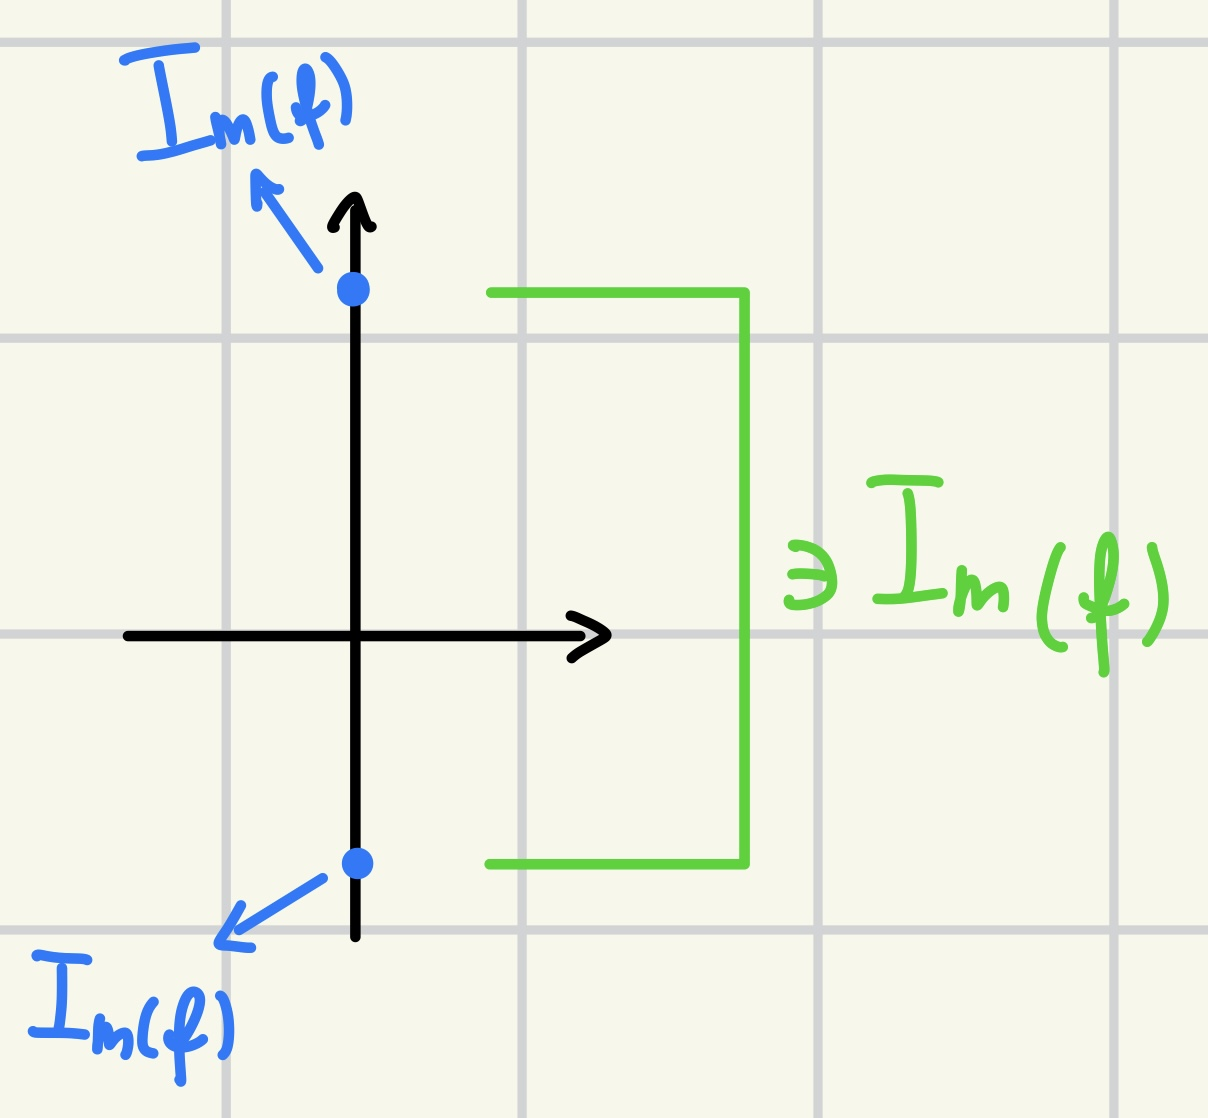
\includegraphics[width=10em]{./images/valori_intermedi.jpg}
\end{figure}
\FloatBarrier

\section{Proprietà della parte intera}
\subsection{Enunciato}
$\forall x \in \R$ $\exists !$ $ n \in \Z$ t.c. $ n \leq x < n + 1$\\
\textbf{N.B.} $n$ è detto parte intera di $x$ $\rightarrow$ $n = \lfloor x \rfloor$

\section{Teorema "Ponte" o limiti mediante successioni}
\subsection{Enunciato}
$f:A \subset \R \rightarrow \R$, $x_0 \in \Rext$ di accumulazione per $A$.\\
\[
\Rightarrow \lim\limits_{x \to x_0}f(x) = l(\in \Rext) \iff \forall \text{successione } a_n \in A \setminus \{x_0\}/\lim\limits_{n \to + \infty}a_n = x_0 \text{, si ha che } \lim\limits_{n \to + \infty} f(a_n)=l
\]
\subsection{Dimostrazione}
"$\Rightarrow$" segue dal teorema di sostituzione dei limiti\\
"$\Leftarrow$" va dimostrato direttamente.

\section{Teorema degli Zeri}
\subsection{Enunciato}
$f:[a, b] \rightarrow \R$, $f$ continua su $[a, b]$ e $f(a)f(b) <0$.
\[
\Rightarrow \exists \overline{x} \in (a,b) / f(\overline{x}) = 0
\]
\subsection{Dimostrazione (metodo dicotomico)}
Suppongo $f(a) < 0 < f(b)$\\
Sia $c=\frac{a+b}{2}$. Calcolo $f(c)$:\\
\begin{enumerate}
    \item[1)] Se $f(c) = 0 \Rightarrow$ la tesi è vera con $\overline{x} = c$ \\
    \item[2)] Se $f(c) < 0 \Rightarrow$ pongo $a_1 = c$, $b_1 = b$ e ho $f(a_1) < 0 < f(b_1)$ \\
    \item[3)] Se $f(c) > 0 \Rightarrow$ pongo $a_1 = a$, $b_1 = c$ e ho $f(a_1) < 0 < f(b_1)$ 
\end{enumerate}

Nei casi 2) e 3): possiamo ripetere il procedimento su $[a_1, b_1]$:\\
Calcolo $c_1 = \frac{a_1 + b_1}{2};$ Valuto $f(c_1)$\\
\begin{enumerate}
    \item[1)] Se $f(c_1) = 0 \Rightarrow$ la tesi è vera con $\overline{x} = c_1$\\
    \item[2)] e 3) come sopra. 
\end{enumerate}

Procedo in tal modo, per induzione, definendo $a_n$, $b_n$, $a \leq a_n < b_n \leq b$ e $f(a_n) < 0 < f(b_n)$.\\
Osservo che $b_1 - a_1 = \frac{b-a}{2}; b_2-a_2 = \frac{b_1-a_1}{2} = \frac{b-a}{4}...=b_n - a_n = \frac{b-a}{2^n}, n \geq 1$\\
Inoltre per costruzione, $a_n < a_n+1$(deb. crescente) $b_{n+1} \leq b_n$(deb. crescente).\\
Per il teorema sui limiti delle funzione monotone:\\
\hSpace $\lim\limits_{n \to + \infty}a_n = l \in [a,b] (a_n \leq a_n \leq b)$\\
\hSpace $\lim\limits_{n \to + \infty}b_n = m \in [a,b] (a \leq b_n \leq b)$\\
D'altra parte, $\lim\limits_{n \to + \infty}(b_n - a_n) = \lim\limits_{n \to + \infty}\frac{b-a}{2^n} = 0$\\
Ma $\lim\limits_{n \to + \infty} (b_n - a_n) = m - l \Rightarrow l = m$.\\
Ricordiamo ora che $f(a_n) < 0 < f(b_n)$ e quindi che: $f(a_n) < f(l) < f(b_n)$\\
\vSpace
D'altra parte per il teorema del confronto, da $f(a_n) < 0$ segue $\lim\limits_{n \to + \infty}f(a_n) \leq 0 \Rightarrow f(l) \leq 0$\\
Infine, per il teorema del confronto, da $f(b_n) > 0 $ segue $\lim\limits_{n \to + \infty}f(b_n) \geq 0 \Rightarrow f(l) \geq 0$.\\
Pertanto $0 \leq f(l) \leq 0 \Rightarrow f(l) = 0$ e la tesi segue $(\overline{x} = l)$

\section{Principio di sostituzione degli infiniti di ordine inferiore}
\subsection{Enunciato}
$f, g, f_1, g_1,$ sono infinite per $ x \to x_0$.\\
$f_1$ è infinito di ordine inferiore a $f$,\\
$g_1$ è infinito di ordine inderiore a $g$ per $x \to x_0$.
\[
\Rightarrow (\lim\limits_{x \to x_0}\frac{f(x)+f_1(x)}{g(x)+g_1(x)} \text{esiste } \iff \lim\limits_{x \to x_0}\frac{f(x)}{g(x)} \text{esiste})\text{ ed in tal caso sono uguali fra loro.}
\]
\subsection{Dimostrazione (Traccia)}
\[\frac{f(x)+f_1(x)}{g(x)+g_1(x)} = \frac{f(x)(1 + \frac{f_1(x)}{f(x)})}{g(x)(g(x) + \frac{g_1(x)}{g(x)})}\]

\section{! Condizione necessaria del primo ordine per punti estremali interni}
\end{flushleft}
\end{document}